%\documentclass[journal]{vgtc}                % final (journal style)
\documentclass[review,journal]{vgtc}         % review (journal style)
%\documentclass[widereview]{vgtc}             % wide-spaced review
%\documentclass[preprint,journal]{vgtc}       % preprint (journal style)
%\documentclass[electronic,journal]{vgtc}     % electronic version, journal

%% Uncomment one of the lines above depending on where your paper is
%% in the conference process. ``review'' and ``widereview'' are for review
%% submission, ``preprint'' is for pre-publication, and the final version
%% doesn't use a specific qualifier. Further, ``electronic'' includes
%% hyperreferences for more convenient online viewing.

%% Please use one of the ``review'' options in combination with the
%% assigned online id (see below) ONLY if your paper uses a double blind
%% review process. Some conferences, like IEEE Vis and InfoVis, have NOT
%% in the past.

%% Please note that the use of figures other than the optional teaser is not permitted on the first page
%% of the journal version.  Figures should begin on the second page and be
%% in CMYK or Grey scale format, otherwise, colour shifting may occur
%% during the printing process.  Papers submitted with figures other than the optional teaser on the
%% first page will be refused.

%% These three lines bring in essential packages: ``mathptmx'' for Type 1
%% typefaces, ``graphicx'' for inclusion of EPS figures. and ``times''
%% for proper handling of the times font family.

\usepackage{mathptmx}
\usepackage{graphicx}
\usepackage{times}
\usepackage{xspace}
\usepackage{amssymb}

% \usepackage[onecolumn]{multicol}

%% algorithm packages (llins)
\usepackage{algorithm}
\usepackage{microtype}
\usepackage{algpseudocode}

%% We encourage the use of mathptmx for consistent usage of times font
%% throughout the proceedings. However, if you encounter conflicts
%% with other math-related packages, you may want to disable it.

%% This turns references into clickable hyperlinks.
\usepackage[bookmarks,backref=true,linkcolor=black]{hyperref} %,colorlinks
\hypersetup{
  pdfauthor = {},
  pdftitle = {},
  pdfsubject = {},
  pdfkeywords = {},
  colorlinks=true,
  linkcolor= black,
  citecolor= black,
  pageanchor=true,
  urlcolor = black,
  plainpages = false,
  linktocpage
}

%% If you are submitting a paper to a conference for review with a double
%% blind reviewing process, please replace the value ``0'' below with your
%% OnlineID. Otherwise, you may safely leave it at ``0''.
\onlineid{}

%% declare the category of your paper, only shown in review mode
\vgtccategory{Research}

%% allow for this line if you want the electronic option to work properly
\vgtcinsertpkg

%% In preprint mode you may define your own headline.
%\preprinttext{To appear in an IEEE VGTC sponsored conference.}

%% Paper title.

\title{RCloud: Integrating Exploratory Visualization, Analysis and Deployment}

% DevOps for Visual Analysis and Data Science

%% This is how authors are specified in the journal style

%% indicate IEEE Member or Student Member in form indicated below
\author{Stephen North and Carlos Scheidegger and Simon Urbanek and
  Gordon Woodhull}

\authorfooter{
%% insert punctuation at end of each item
}

%other entries to be set up for journal
% \shortauthortitle{Biv \MakeLowercase{\textit{et al.}}: Global Illumination for Fun and Profit}
%\shortauthortitle{Firstauthor \MakeLowercase{\textit{et al.}}: Paper Title}

%% Abstract section.
\abstract{ Consider the emerging role of a data science team within an
  organization. Individual data scientists and statisticians usually
  work on loosely related problems, and must devise effective ways to 
  share their findings and to move results from exploratory data analysis
  to automated diagnostics and reports deployed for wider consumption.
  There are two problems with the current
  practice. First, there are gaps in this workflow: EDA is performed
  with one set of tools, and automated reports and deployments with another.
  Second, EDA environments often assume a single-developer perspective,
  while data scientist teams could greatly benefit from easier sharing of
  scripts and data feeds, experiments, annotations, and automated
  recommendations, which are well beyond what traditional version control
  systems provide.  \todo{sell idea, not system} In this paper, we propose RCloud, a system that supports
  collaborative data analysis, visualization and web deployment. We will
  discuss the design decisions, tradeoffs and limitations, and compare RCloud
  to other current proposals.
} % end of abstract

%% Keywords that describe your work. Will show as 'Index Terms' in journal
%% please capitalize first letter and insert punctuation after last keyword
\keywords{Some, Keywords, Here}

%% \CCScatlist{ % not used in journal version
%%  \CCScat{K.6.1}{Management of Computing and Information Systems}%
%% {Project and People Management}{Life Cycle};
%%  \CCScat{K.7.m}{The Computing Profession}{Miscellaneous}{Ethics}
%% }

%% Uncomment below to include a teaser figure.
\teaser{
  \centering
  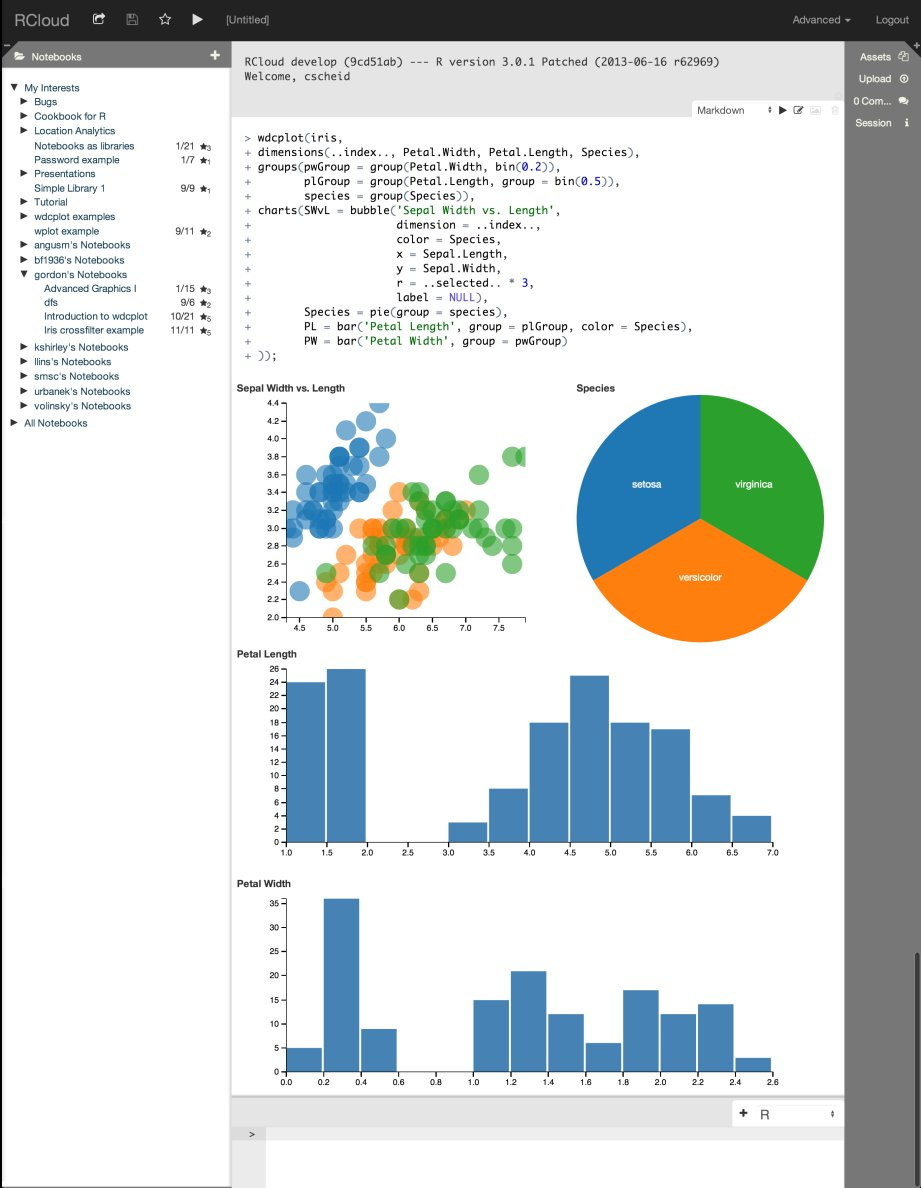
\includegraphics[width=.3\linewidth]{fig/screenshots/wdcplotsmall.jpg}
  %% 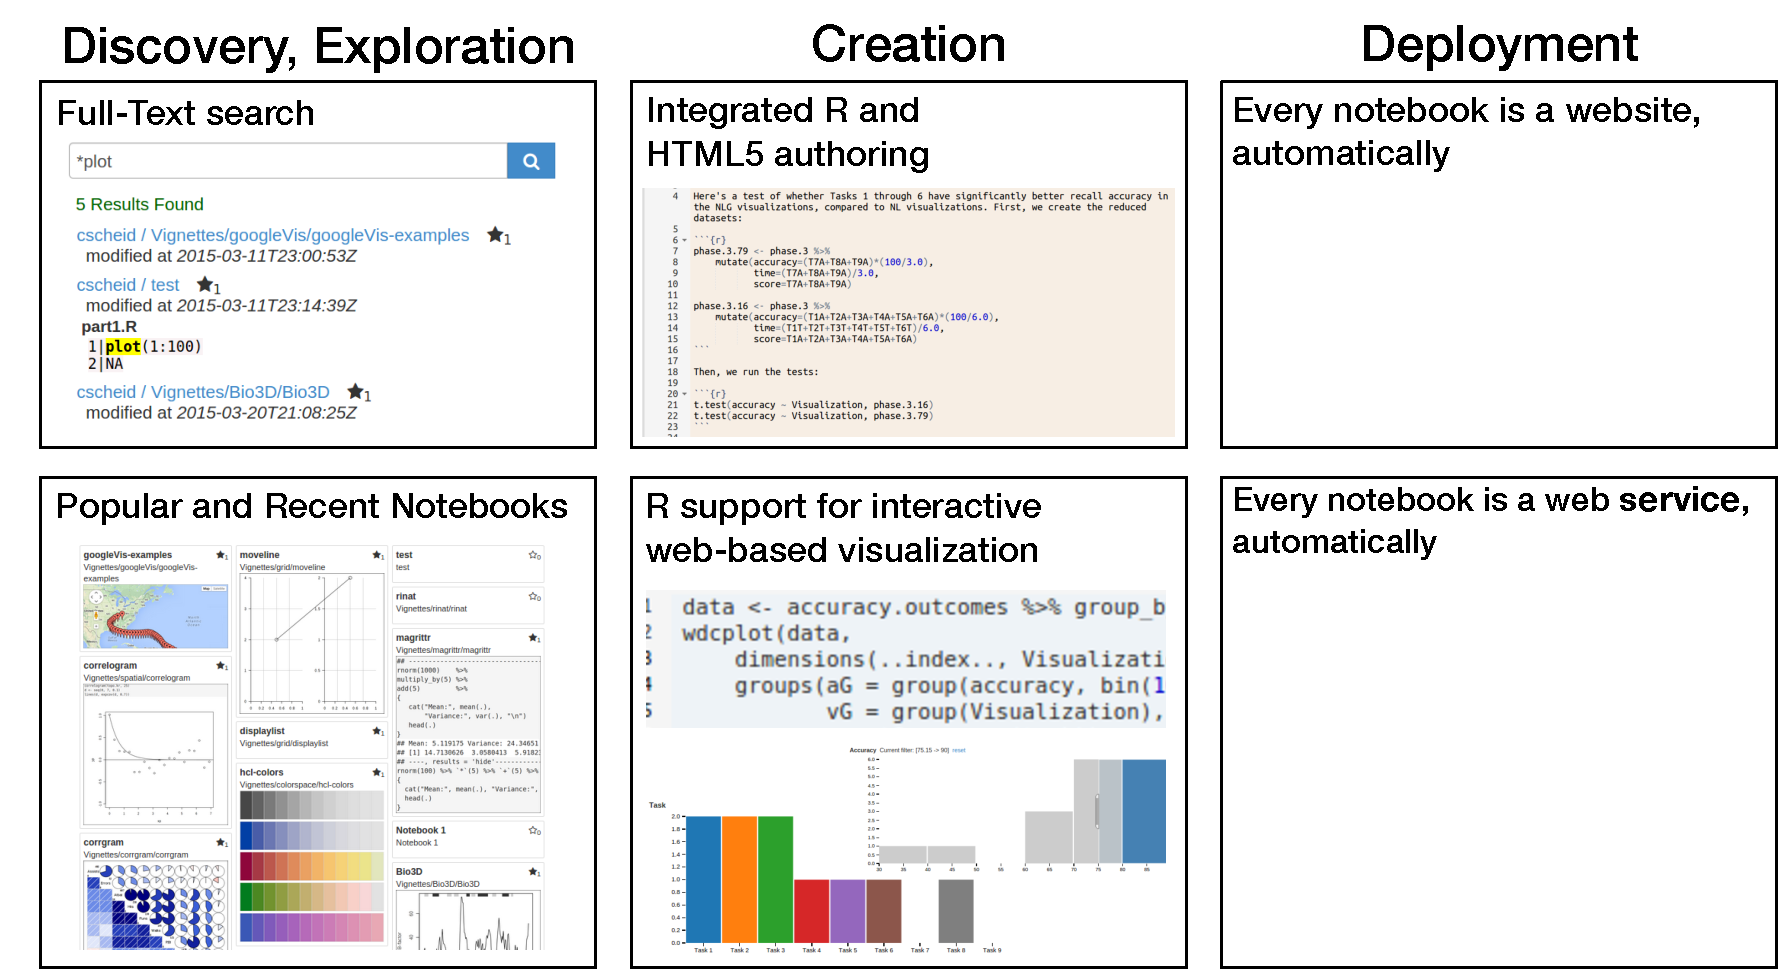
\includegraphics[width=.9\linewidth]{figs/teaser.jpg}
  % \vspace{-.5em}
  \caption{Left: RCloud integration of HTML5 visualization libraries such
    as D3~\cite{Bostock:2011:DDD} and Crossfilter~\cite{Square:2014:CFM}.
  }
% \vspace{-.5em}
}

%% Uncomment below to disable the manuscript note
%\renewcommand{\manuscriptnotetxt}{}

%% Copyright space is enabled by default as required by guidelines.
%% It is disabled by the 'review' option or via the following command:
% \nocopyrightspace

%
% Useful Macros 
%

\newcommand{\eg}{e.g.\xspace} % e.g. and i.e. ARE NOT ITALIC!!
\newcommand{\ie}{i.e.\xspace}
\newcommand{\todo}[1]{\textcolor{red}{#1}}

\newcommand{\stephen}[1]{{\color{green} SN: [{#1}]}}
\newcommand{\carlos}[1]{{\color{cyan} CS: [{#1}]}}
\newcommand{\simon}[1]{{\color{red} SU: [{#1}]}}
\newcommand{\gordon}[1]{{\color{violet} GW: [{#1}]}}

%% \renewcommand{\stephen}[1]{}
%% \renewcommand{\carlos}[1]{}
%% \renewcommand{\simon}[1]{}
%% \renewcommand{\gordon}[1]{}


%%%%%%%%%%%%%%%%%%%%%%%%%%%%%%%%%%%%%%%%%%%%%%%%%%%%%%%
%%%%%%%%%%%%%%%%%%%%%% ALGORITHM %%%%%%%%%%%%%%%%%%%%%%
%%%%%%%%%%%%%%%%%%%%%%%%%%%%%%%%%%%%%%%%%%%%%%%%%%%%%%%

\renewcommand{\algorithmicthen}{}

% aux. commands

%%%%%%%%%%%%%%%%%%%%%%%%%%%%%%%%%%%%%%%%%%%%%%%%%%%%%%%%%%%%%%%%
%%%%%%%%%%%%%%%%%%%%%% START OF THE PAPER %%%%%%%%%%%%%%%%%%%%%%
%%%%%%%%%%%%%%%%%%%%%%%%%%%%%%%%%%%%%%%%%%%%%%%%%%%%%%%%%%%%%%%%%

\begin{document}

%% The ``\maketitle'' command must be the first command after the
%% ``\begin{document}'' command. It prepares and prints the title block.

%% the only exception to this rule is the \firstsection command

\firstsection{Introduction}

\maketitle

\todo{Points we want to make."Coordination is done by meetings" "how do you trace an automated alert back to an EDA environment ?"}

% What's the area
Consider the emerging role of a data science team within an
organization \cite{Keim:2008:VAS}.

% How do people do it today?
Individual data scientists and statisticians usually
work on loosely related problems, and must devise effective ways to 
share their findings and to move results from exploratory data analysis
to automated diagnostics and reports deployed for wider consumption.
They generally rely on a patchwork of resources that are shared informally,
or at best, through systems that attack some of the tasks or functions in
the data analysis workcycle.

% Why does this not work?
There are two problems with the current
practice. First, there are gaps in this workflow:
Exploratory Data Analysis (EDA) is performed with one set of tools,
and automated reports and deployments with another.
Second, EDA environments often assume a single-developer perspective,
while data scientist teams could greatly benefit from easier sharing of
scripts, data sets, data feeds, experiments, annotations, and automated
recommendations, which are well beyond what traditional version control systems provide. 

% What are we going to do about this?
\todo{Sell idea, not system} In this paper, we investigate the hypothesis
that the practice of visual analytics can advance by adopting techniques
from information retrieval and collaborative computer, formally supported
within the computing environment. To investigate this, we propose RCloud,
a system that supports collaborative data analysis, visualization and
web deployment. We will discuss the design decisions, tradeoffs and
limitations, and compare RCloud to other current proposals.

\todo{Define the requirements for the system}
\begin{itemize}
\item Technology transfer. Things developed by analysts need to become accessible in the production environment and should be supported in the environment, making it easy to push new features, experiments, etc.
\item Dasboarding. There should be a mode in which people can operate the experiments without coding. At times code has to be written because some things cannot be done any other way but other people must not ever see code because their eyes will fall out.
\item Version control as a primary concept in the repository. Need to control the visibility of 
\item Modern interactive technologies. People want to interact with data to explore it. Scalable technologies like crossfilter exist. Want to support those in the context of an R environment. Need to support full 2-way communication between computing in the cloud and interaction on the web.
\item Other requirements e.g. Kandel's user study. Not our contribution but things we must address, mentioned in related work section. Heer/Agrawala design considerations for collaborative visual analytics.
\end{itemize}

% What is the scope of our solution?
Our investigation focuses on the R language \cite{RCoreTeam:2013:R}
for statistical computing and graphics. R is one of the most popular
systems for ...

% We want our solution to play well with the rest of the ecosystem
R has developed a complex ecosystem of compatible packages, software
tools and other resources. For example there are packages that make
it convenient to execute map-reduce programs, generate web interfaces,

\section{Related Work}

Kandel et al. argue in their review of data wrangling work that data
cleaning, wrangling and transformation is a major part of exploratory
analysis and visualization~\cite{Kandel:2011:RDI}. Although RCloud
does not by itself include modules specific to data cleaning and
wrangling, we note from internal experience that these cleaning
scripts themselves tend to change over time. RCloud addresses this
issue by providing easy publishing of data-cleaning notebooks as web
services, which reduces the total data-cleaning effort across an
organization.

Kandel et al.'s interview study points out the typical ``explore'',
``model'', ``report'' cycle in enterprise data
analysis~\cite{Kandel:2012:EDA}. There are many discontinuities in
this cycle that cost time and effort to overcome. RCloud seeks to
reduce this impedance mismatch. They also point out that larger teams
are becoming more common in data analysis, that supporting
collaboration is a difficult and important problem, and that sharing
and versioning of data sources and artifacts is hindered by current
technology in practice. ``We found that analysts typically did not
share scripts with each other. Scripts that were shared were
disseminated similarly to intermediate data: either through shared
drives or email. Analysts rarely stored their analytic code in source
control.'' Their work points to the opportunity for better technology
to support collaboration and sharing by data analysis teams.

Heer and Agarwala identify many design considerations for
collaborative visual analytics~\cite{Heer:2008:DCF}. \emph{Starring},
the means for signaling interest in notebooks, described in
Section~\ref{sec:starring}, addresses social-psychological incentives,
recommendation, and voting and ranking. RCloud's integrated deployment
mechanism, described in Section~\ref{sec:deployment}, addresses cost of
integration, content export, presentation and view sharing. Notebooks,
and the integrated version control system for them, described in
Section~\ref{sec:notebooks}, address modularity and granularity, and
artifact histories.

Manyeyes \cite{Viegas:2007:MAS} was a landmark system for the integration
of social media with visualization and data publishing. We build on this
work by defining a rich interface for collaboration about code and for
operating on metadata.

The need for integrating statistics and visualization has been
highlighted in previous studies and is widely understood by
various technical communities \cite{Perer:2008:ISA}

There has been noteworthy work on specific techniques such as
social bookmarking \cite{Millen:2006:DSB} \cite{Heer:2007:VAV}
and crowdsourcing \cite{Fast:2014:ECS} to support collaborative
or social development or analysis processes.
Similarly, there are computational methods to support high
performance execution in incremental code development
environments \cite{Guo:2010:TPI}.
Our goal is to define an environment in which many such
techniques may be integrated and made available to a broad community.

VisMashup
\cite{Santos:2009:VST}

Crowdlabs
\cite{Mates:2011:CSA}

Our work has been inspired by and benefited from other proposals
to improve data analysis environments and processes,
including RStudio \cite{RStudio:2013:SWA},
R packages such as Markdown \cite{Allaire:2014:MMR},
knitr \cite{Xie:2013:DDW}
and Shiny \cite{RStudio:2013:SWA},
and iPython notebooks \cite{Perez:2007:IAS}
to name a few. RStudio aims at providing an integrated development environment
for R programming, with support for publishing code in packages. Markdown,
knitR and Shiny provide R with sophisticated reporting capabilities, including
interactive web interfaces. IPython \cite{Perez:2007:IAS}
shares many of our goals, such as providing a comprehensive environment
for analysis and programming, with sharable documents on the web.

One overall goal is to reduce the gap between implementors and deployers
of technology. Don't want a team of 20 IT people to support 5 data scientists.

% devops for data science.

\section{System Architecture}

\begin{figure}
\hspace{-0.08\linewidth}
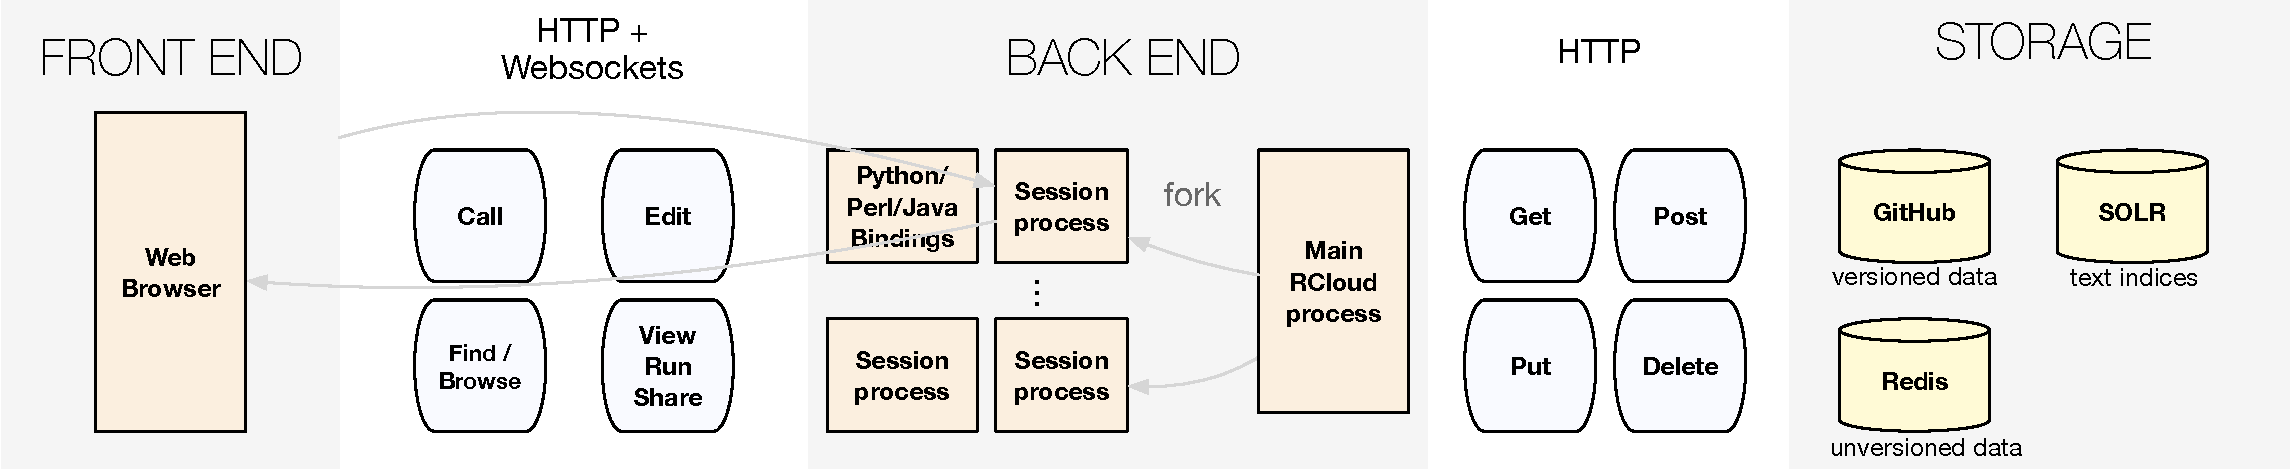
\includegraphics[width=1.1\linewidth]{fig/system/system.pdf}
\caption{\label{fig:system}A diagram of RCloud's architecture}
\end{figure}

Design for cloud-friendly? This goes back to the point in the
introduction about playing nice with the rest of the ecosystem.

\section{System Design}

\subsection{Notebooks\label{sec:notebooks}}

\subsection{Reputation and Interest: starring\label{sec:starring}}

\subsection{Deployment of notebooks\label{sec:deployment}}

Notebooks as versioned subroutines, web services.

Notebooks by default are visible by the entire organization: there
exists a URL for every notebook in RCloud. This is deliberate. As
pointed out by Wattenberg and Kriss~\cite{Wattenberg:2011:DFS}, broad
access to analysis outputs (in their case, in the form of NameVoyager)
increases long-term engagement partly by the crossreferences in the
web. Our main RCloud deployment is only visible inside an intranet,
but we have nevertheless found anecdotal support for this theory by
noticing links to RCloud notebooks in internal discussion fora and
mailing lists.

\subsection{Technologies: R, Python, HTML5, interactive notebooks, etc.}

How do we do things that are not trivial to do with IPython (for example)

dcplot. two-way communication between between backend session and
frontend session.

\section{Case Studies}

\section{Lessons Learned}

\section{Discussion and Limitations}

What are the decisions and ideas that are central to this paper?

discussion about binding times, running vs.caching.
transparent vs. explicit operations done by programmers

% limitations
Previous studies have pointed out difficulties in achieving the flexibility,
scalability and maintainability expected of production software with experimental
code created by data analysts.
These properties cannot be ensured by any programming environment,
but suitable tools can help well-motivated analysts and programmers to create
robust applications with much less effort.

Asynchronous collaborative visual analytics
(ACVA)~\cite{Chen:2011:SEC}. This paper addresses visualization
\emph{of} the ACVA process. It will be important when we talk about
recommendation systems, and navigation of the set of notebooks, etc.

\bibliographystyle{abbrv}

\bibliography{paper}
\end{document}
